\subsection{Workshop}
\label{workshops}

Tjora (2012) påpeker at valg av metode for datagenerering må reflektere hva man faktisk ønsker å finne ut, og at effektivitet bør vektlegges. “Datagenereringen må kunne frambringe mest mulig relevant og pålitelig informasjon uten unødig bruk av forskeres og deltakeres tid og ressurser”.
I tråd med \ref{chp: medvirkning} og \ref{chp:dd}, ønsket vi en brukersentrert designprosess, hvor brukerene medvirket gjennom en \emph{deltagende design workshop}.
En slik workshop åpner for at utviklere, bedriftsrepresentanter og brukere kan jobbe sammen for å avdekke utfordringer og løsninger på en svært produktiv måte. Dette vil være mest effektivt tidlig i designprosessen, da idèer ikke hemmes av eksisterende kode eller annen infrastruktur (Gaffney, 1999).

\subsubsection{Kontekst}
Vi gjennomførte to workshoper over to dager. Disse ble holdt på NSEP brukbarhetslab (Norsk senter for elektronisk pasientjournal) ved St. Olavs Hospital. Brukbarhetslaben er bygget for å kunne observere og teste mobile helsetjenester \cite{NSEP}.
Som Alsos og Dahl (2008) beskriver, vil sykehus ofte ha strenge restriksjoner mot å tillatte eksperimentelle forsøk, da slike forsøk kan ha en påtrengende effekt på det pågående arbeidet. I tillegg kan opptak av observasjoner være forbudt, da pasientinformasjon er konfidensielt. Ved testing i brukbarhetslab kan man fokusere på relevante bruksområder, og kontrollere faktorer irrelevante for evaluering av løsningen \cite{Alsos08}. På grunn av tidsbegrensning var det derfor naturlig å benytte brukbarhetslaben som testmiljø.   


\subsubsection{Artefakter}
\begin{figure}[H]
\centering
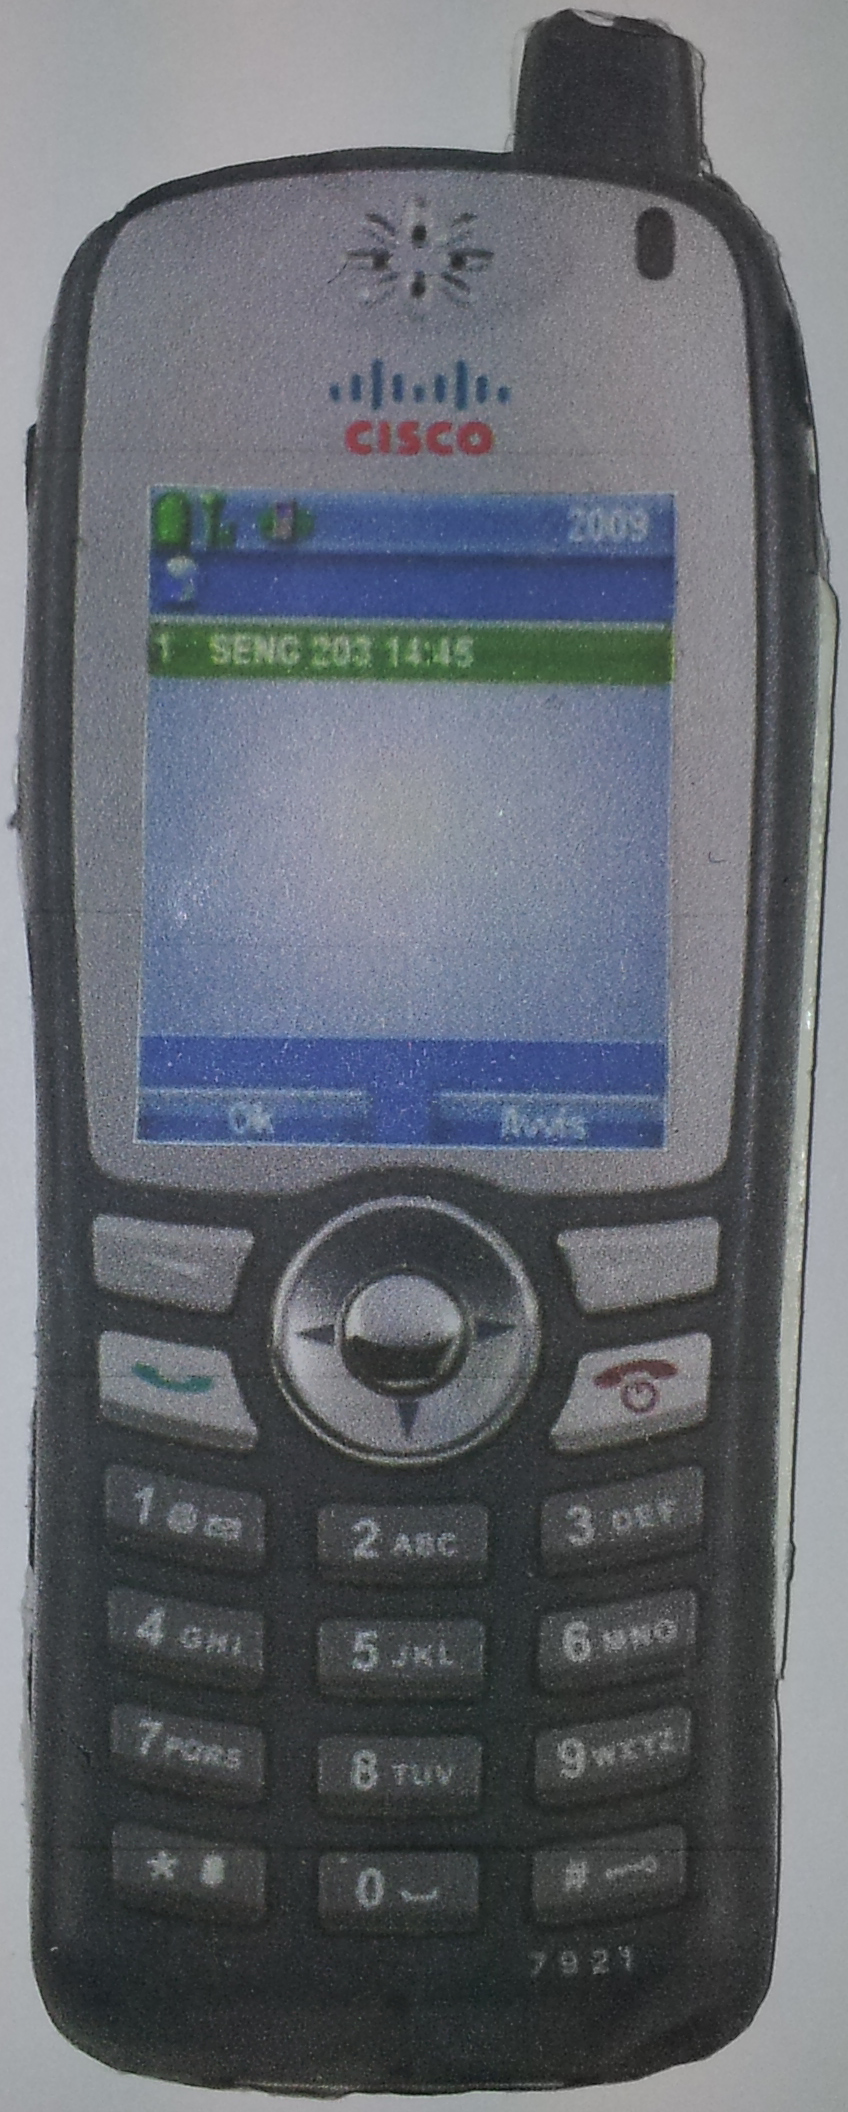
\includegraphics[scale=0.1]{mock-up_Telefon.jpg}
\caption{Mock-up av telefonen sykepleierene bruker i dag}
\label{mock-up_Telefon}
\end{figure}

\begin{figure}[H]
\centering
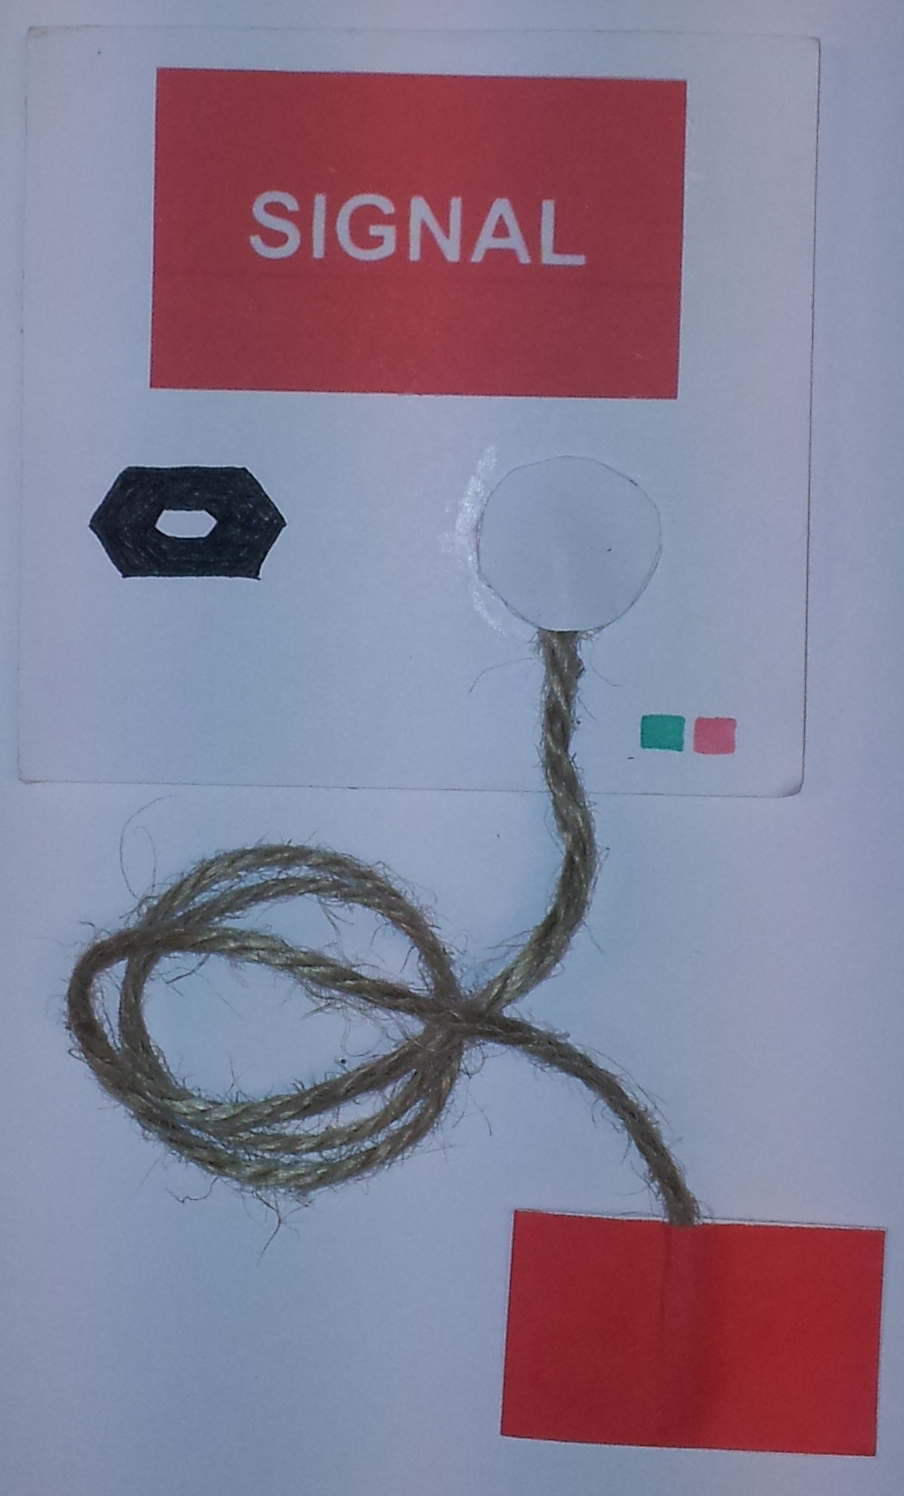
\includegraphics[scale=0.1]{mock-up_PasientPanel.jpg}
\caption{Mock-up av panelet hvor snoren pasienten kan trekke i er festet}
\label{mock-up_PasientPanel}
\end{figure}

\begin{figure}[H]
\centering
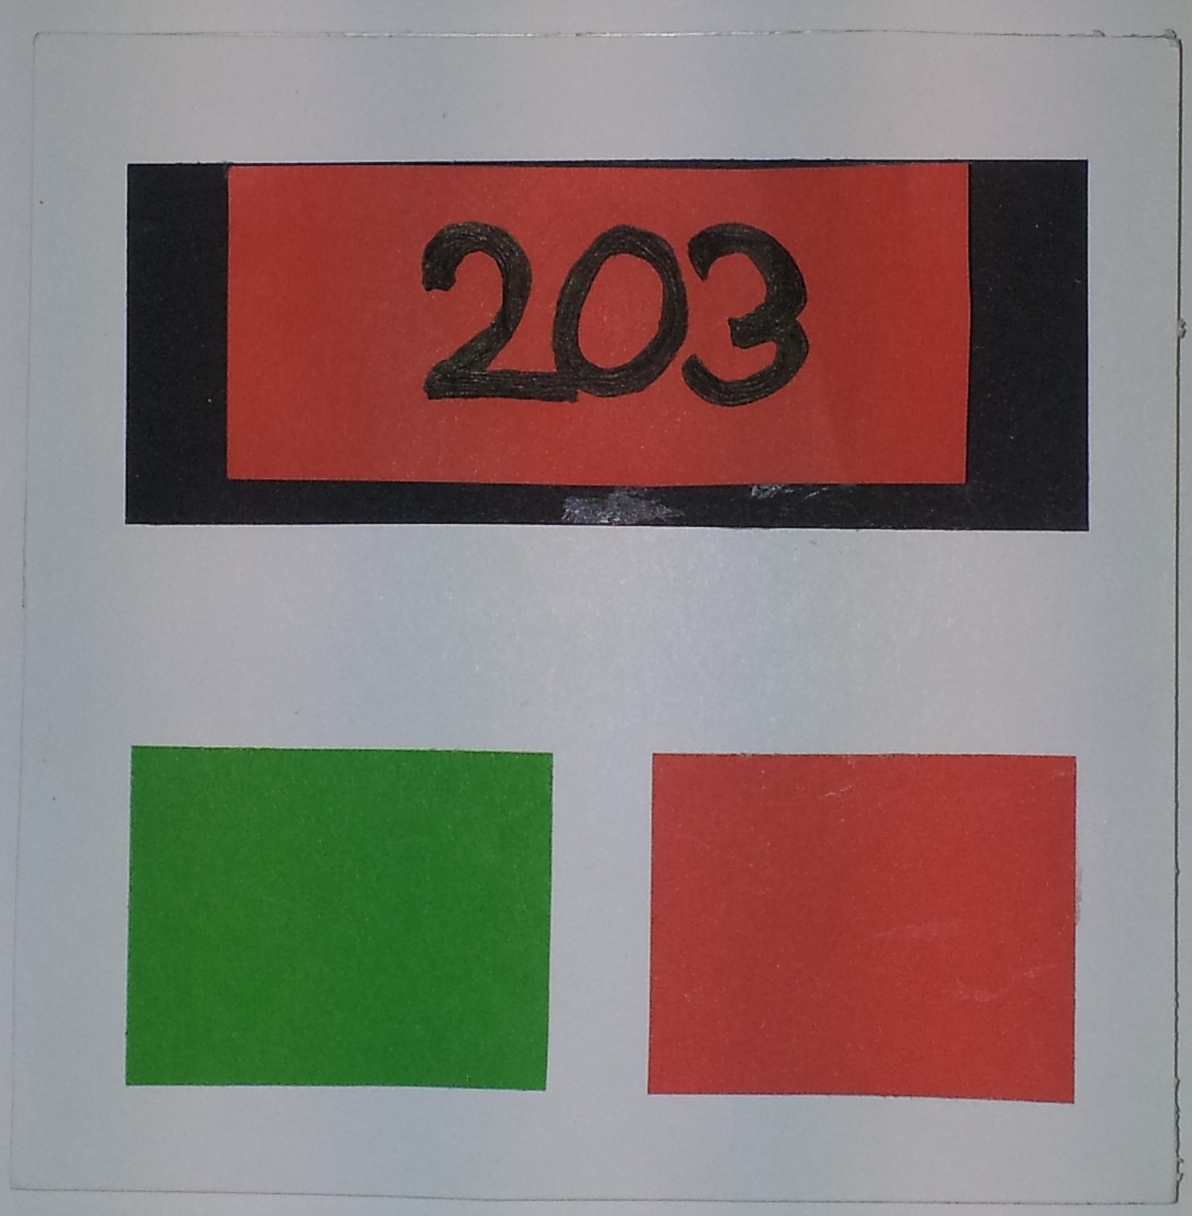
\includegraphics[scale=0.1]{mock-up_RomPanel.jpg}
\caption{Mock-up av panelet hvor sykepleiere trykker på den grønne knappen for å vise sin tilstedeværelse. Romnummer hvor pasientsignal er aktivt vil vises, her rom 203}
\label{mock-up_RomPanel}
\end{figure}

\begin{figure}[H]
\centering
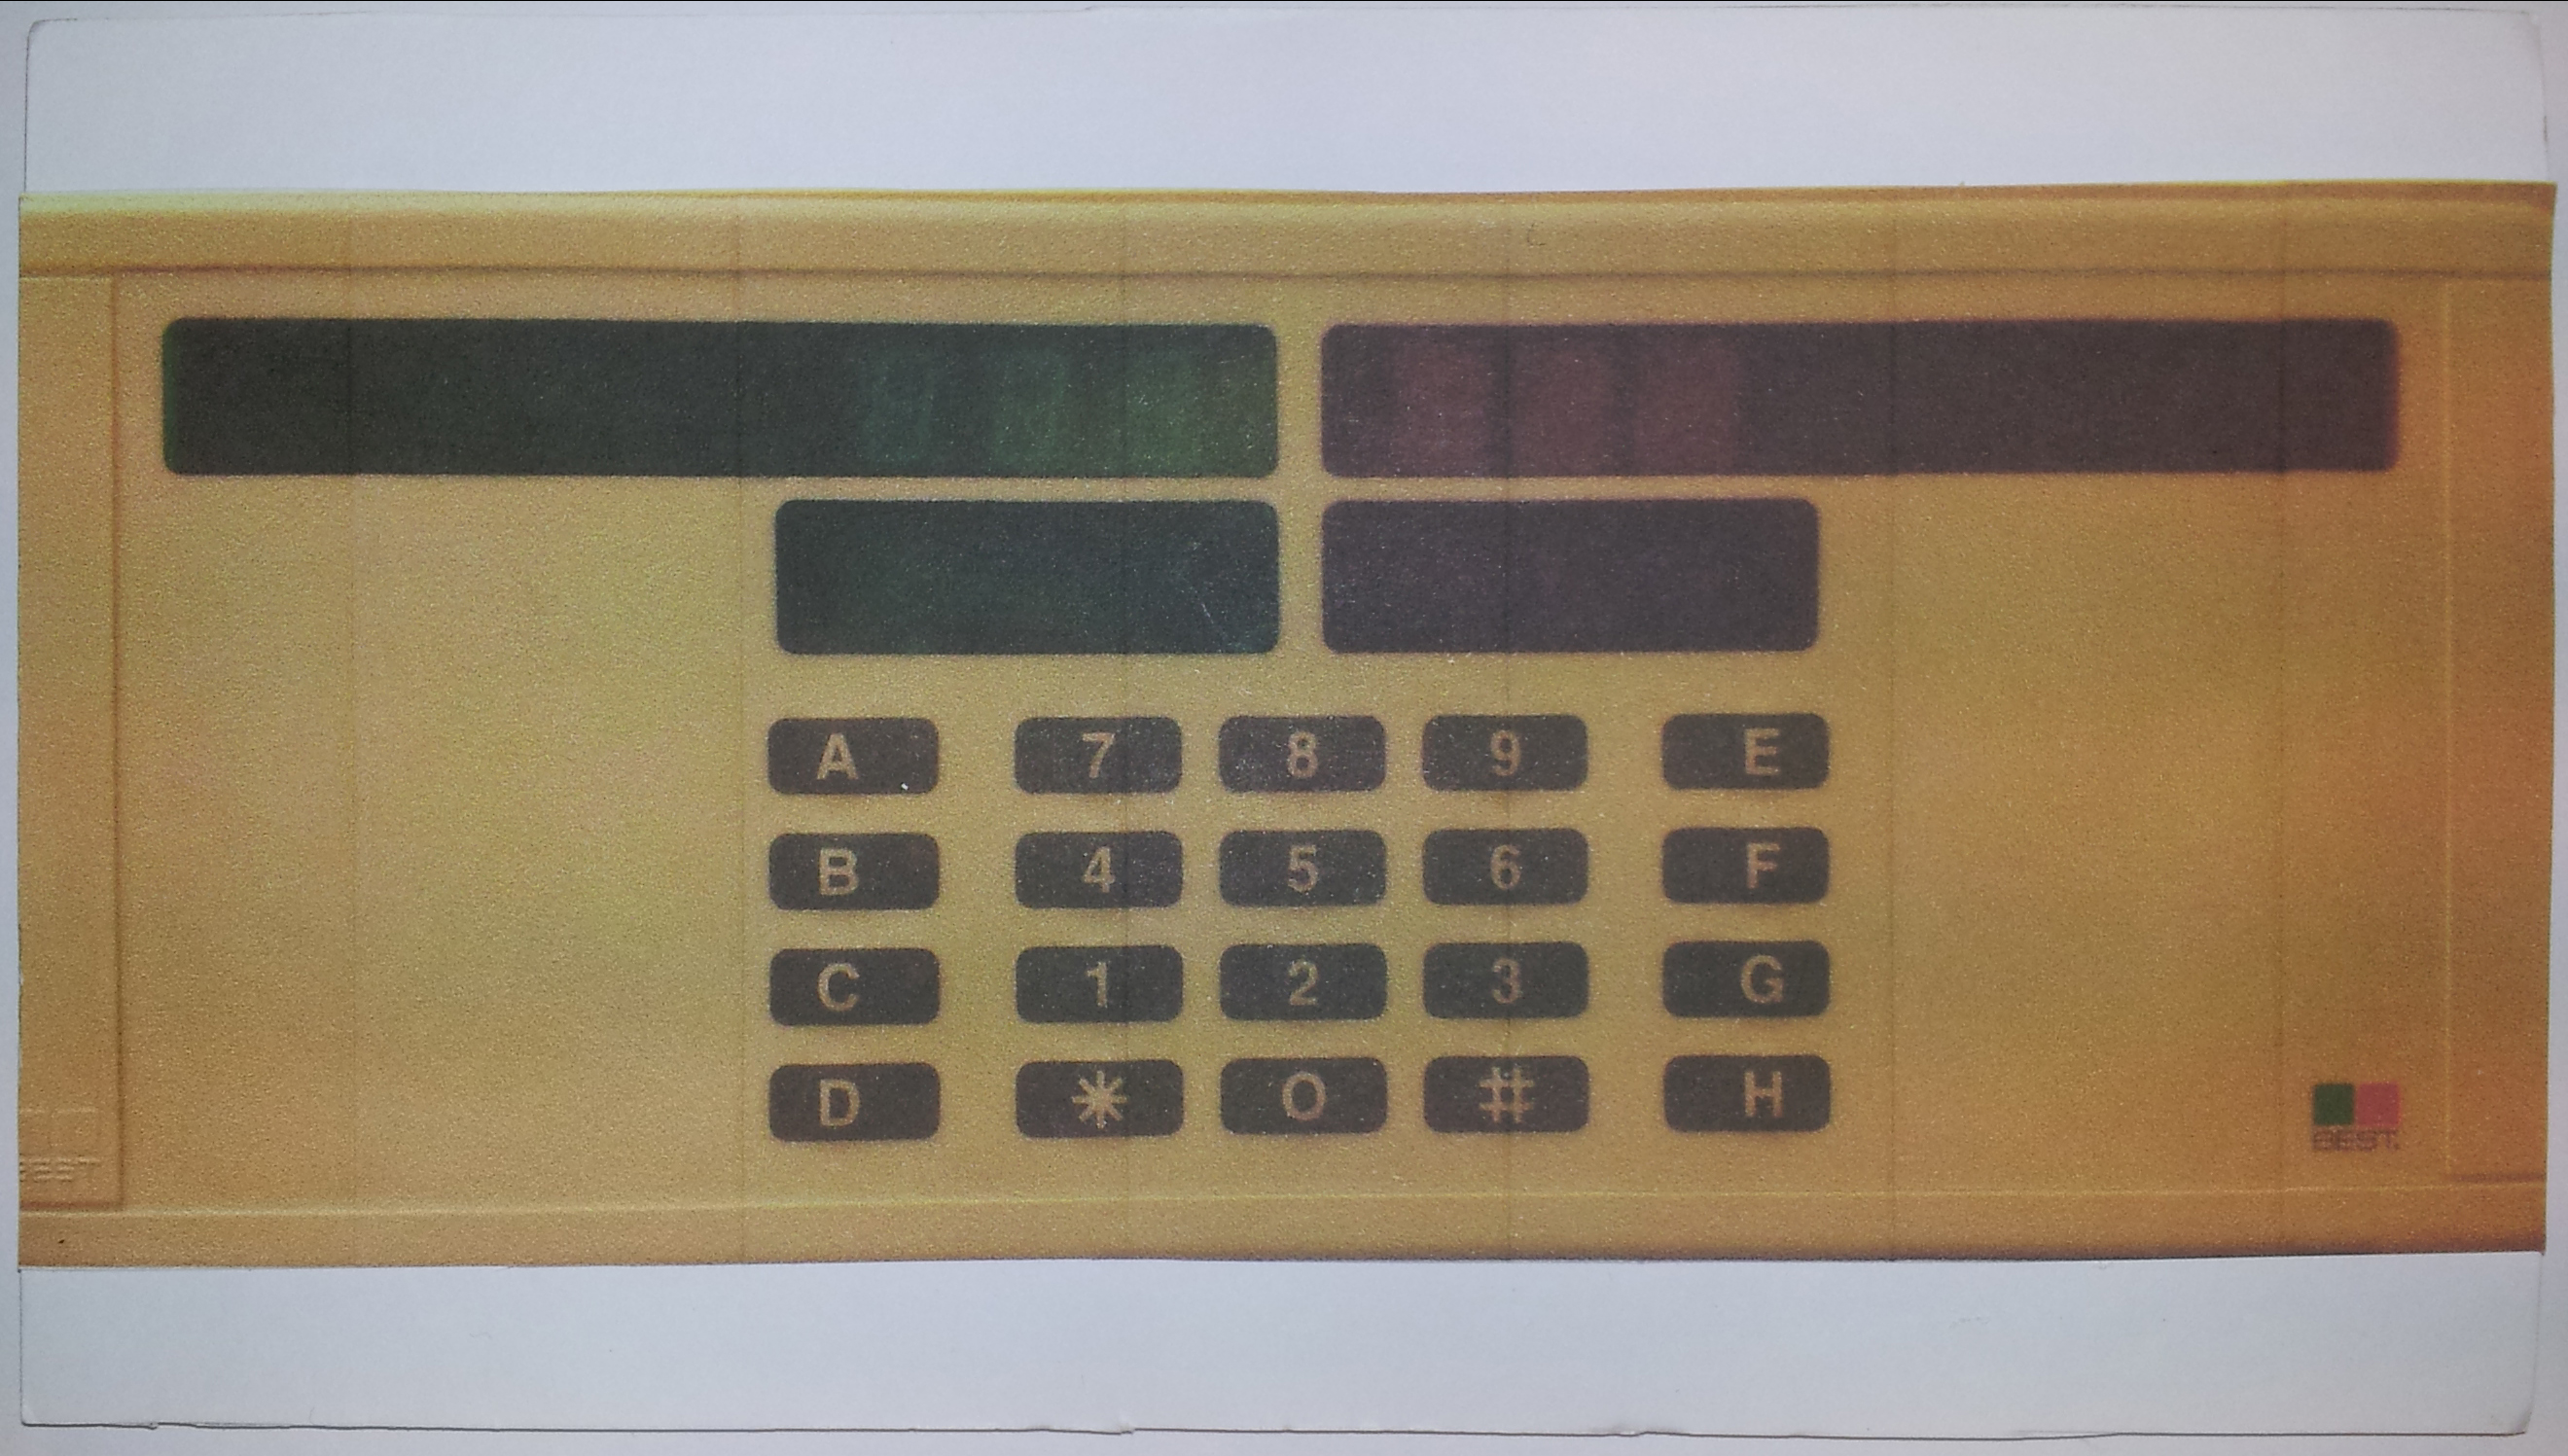
\includegraphics[scale=0.1]{mock-up_VaktPanel.jpg}
\caption{Mock-up av panelet plassert ved vaktposen på sengetunet. Her vises romnummer hvor pasientsignal er aktivt samt romnummer hvor sykepleiere har registrert tilstedeværelse}
\label{mock-up_VaktPanel}
\end{figure}

\subsubsection{Scenarioer}
Som beskrevet av Svanæs og Seland (2004), er rollespill med bruk av lavnivå-protoype en god måte å få brukere og utviklere "opp av stolen", og gjør det mulig å utforske designkonsepter med brukere i en tidlig fase. Scenario-basert design, belyst av Bardram (2000), er nyttig i situasjoner hvor man ikke har en detaljert oppfattelse av nøyaktig hvilke arbeidsaktiviteter som skal støttes, og på hvilken måte. Denne designprosessen har to karakteristikker, (1) man ønsker å re-designe de eksisterende måtene å gjøre ting på for å forstå hvordan ting kan gjøres annerledes ved hjelp av et datasystem. Dette starter ofte ved at man undersøker problemene og fordelene med det eksisterende systemet. (2) Deretter starter den kreative prosessen, hvor designeren, med sin tekniske erfaring, og brukeren, med sin arbeids- og organisasjonserfaring, sammen kommer opp med nye ideer. Relevante spørsmål man bør stille seg i en slik prosess er; er disse ideene nyttige? Og hvilke arbeidsaktiviteter støtter de, og hvilke forstyrrer de? Bruk av scenarioer er dermed nyttig fordi de støtter det kreative samspillet mellom designer og bruker, og de besvarer spørsmål om nyttigheten til systemet sammenlignet med arbeidsrutinene i en organisasjon. Det Bardram (2000)\nocite{Bardram00} kaller arbeidsaktivitets-scenarioer, er scenarioer som prøver å få en klarhet i det samarbeidende arbeidet vi ønsker å designe for. 
I tråd med det Bardram (2000) skriver, var det ønskelig å bruke to sett med scenarioer, ett hvor dagens system og arbeidspraksis ble brukt, og ett hvor vi ønsket å teste de ideene vi hadde kommet opp med, og skape en kreativ prosess for videre forslag og innspill fra deltagerne. Det ble tatt utgangspunkt i scenarioer og pasientbeskrivelser i Selseth (2012)\nocite{Selseth12}, med noen endringer for å gjøre de relevante til våre forskningsspørsmål. Scenarioene i sin helhet er vedlagt som en del av tillegg B.

%\begin{adjustbox}{with=\textwith, hight=\texthight}
\begin{table}[H]
%\small
\caption{Overordnet plan for dagen}
%\centering
\begin{tabular}{l|l|l|l|l}
\hline
\textbf{\begin{tabular}[x]{@{}c@{}}Del av\\workshop\end{tabular}} & \textbf{Beskrivelse} & \textbf{Hvor} & \textbf{Tidspunkt} & \textbf{Varighet}\\
\hline
Steg 1 & Informasjon & \begin{tabular}[x]{@{}c@{}}Rundt bord\\/i gangen\end{tabular} & 13:00-13:15 & 15min\\
\hline
Steg 2 & Fokusgruppe med scenarioer & \begin{tabular}[x]{@{}c@{}}Rundt bord\\/i gangen\end{tabular} & 13:15-13:45 & 30min\\
\hline
& \textbf{Pause} & & 13:45-13.50 & 5min\\
\hline
Steg 3 &\begin{tabular}[x]{@{}c@{}} Scenarioer med rollespill\\- uten prototype\end{tabular} & Inne på sengerom & 13:50-14:25 & 35min\\
\hline
Steg 4 &\begin{tabular}[x]{@{}c@{}}Scenarioer med rollespill\\- med prototype\end{tabular} & Inne på sengerom & 14:25-15:00 & 35min\\
\hline
& \textbf{Pause} & & 15:00-15:15 & 15min\\
\hline
Steg 5 & Fokusgruppe/oppsummering & \begin{tabular}[x]{@{}c@{}}Rundt bord\\/i gangen\end{tabular} & 15:15-16:00 & 45min
\end{tabular}
\label{Plan}
\end{table}
%\end{adjustbox} 

\noindent
Som gitt av tabell \ref{Plan}, ble scenarioene delt i tre deler. I steg 2 ønsket vi å avdekke generelle likheter og ulikheter mellom avdelingene, knyttet til ansvarsfordeling og situasjoner hvor det kunne være ønskelig å være utilgjengelig. I første del av steg 3 ønsket vi å avdekke problemer og fordeler med det eksisterende systemet og arbeidspraksis, mens andre del ble relatert til den løsningen vi ønsket å teste. 

\subsubsection{Fokusgruppe}
Fokusgrupper kan være en effektiv form for datagenerering fordi man utvikler intervjudata fra flere informanter samtidig. Informantene kan stimulere hverandre, og dermed få frem mange aspekter av informantenes oppevelser av fenomener de alle kjenner til, og opplevelsen fra fokusgruppen kan være kilde til nye tanker og refleksjoner. For å styre ordet, og sørge for at alle får sagt de ønsker, brukes moderatorer. Disse vil også formulere spørsmål for å sette i gang diskusjoner, og eventuelle oppfølgingsspørsmål \cite{Tjora}. 

\noindent
Første dag var Veronica moderator og Monika assisterende moderator, og motsatt dag to. I tillegg deltok Joakim Klemets som assisterende moderator begge dager. De assisterende moderatorene stilte utfyllende spørsmål ved behov og ønske. Da det ble tatt videoopptak av workshopene var det ikke nødvendig at de assisterende moderatorerene dokumenterte sesjonene. 
Under utspillingen av scenarioene ble kun et par av deltagerene valgt til å delta, mens de andre observerte fra videorommet bak, hvor de hadde fullt innsyn i hva som skjedde under utspillingen. For hvert scenario som ble utspilt, ble det i etterkant gjennomført fokusgruppe slik at alle deltagerene kunne evaluere og  reflektere over de situasjonene som oppsto i scenarioet.


\subsubsection{Videoopptak}
\subsubsection{Deltagere og utførelse}
Det ble i forkant av workshopene sendt mail til de ansvarlige for sykepleierstudentene, med den intensjon å rekruttere studenter gjennom disse. Da påmeldingen gikk sent, ble det behov for å ringe og besøke de ulike sengetunene på St. Olavs Hospital, for å komme i direkte kontakt med studentene. 
Det ble arrangert to like workshoper, WS1 og WS2, med totalt 9 deltagere, se tabell \ref{DeltagereWS}. Alle deltagere og avdelinger er anonymisert, og kolonnen \emph{Notasjon} er brukt for å knytte resultatene til de aktuelle deltagerene. Alle deltagerene var andreårs sykepleierstudenter ved HiST (Høyskolen i Sør-Trøndelag). Da vi hadde behov for alle de påmeldte, var vi ikke i en posisjon hvor vi kunne velge ut deltagere for å få en viss gruppesammensetting. Det at vi kun hadde tilgang til studenter, og ikke arbeidende sykepleiere, medførte at deltagerene hadde begrenset erfaring med systemet, og man kan stille spørsmål til hvorvidt utvalget var representativt. Da studentene er aktuelle fremtidige brukere av systemet vi ønsket å teste, anså vi likevel workshopene som nyttige.

\begin{table}[H]
\begin{tabular}{ |l|l|l|l| }
\hline
\multicolumn{4}{ |c| }{Deltagere ved workshoper} \\
\hline
WS & Deltagere & Avdeling & Notasjon \\ \hline
\multirow{4}{*}{WS1} & S1 & A1 & S1-A1 \\
 & S2 & A2 & S2-A2 \\
 & S3 & A3 & S3-A3 \\
 & S4 & A3 & S4-A3 \\ \hline
\multirow{5}{*}{WS2} & S5 & A3 & S5-A3 \\
 & S6 & A4 & S6-A4 \\
 & S7 & A1 & S7-A1 \\
 & S8 & A5 & S8-A5 \\
 & S9 & A3 & S9-A3 \\ 
\hline
\end{tabular}
\label{DeltagereWS}
\end{table}

\noindent
Innledningsvis til workshopene, se steg 1 i tabell \ref{Plan,} ble det gitt informasjon om prosjektet, forklart hva workshopene ville innebære, og deltagerene signerte informasjonsskriv, se tillegg C. Deretter, i steg 2, ble generelle scenarioer presentert, og deltagerene ble spurt spørsmål vedrørende disse. Hensikten her var å avdekke generell arbeidspraksis rundt ansvarsfordelingen i ulike situasjoner.
Før steg 3 og 4, ble studentene presentert to ulike pasienter, med to ulike sykdomsbilder. Disse var i likhet med scenarioene hentet fra Selseth (2012), hvor kun navnet på den ene pasienten ble endret. Studentene rullerte på å spille de fire scenarioene for hver dag, mens pasientene ble spilt av forskerene. I steg 3, ble to scenarioer utspilt, uten bruk av prototype. Hensikten var å avdekke problemer, utfordringer og fordeler med det eksisterende systemet. Videre i steg 4 ble de samme scenarioene utspilt, men med prototype. Her var det ønskelig at deltagerene evaluerte prototypen og dens funksjonalitet, samtidig som de ble oppfordret til tenke fritt og kreativt om nye, alternative løsninger. Underveis i utspillingen ble deltagerene spurt spørsmål av fasilitator. Veronica hadde rollen som fasilitator under WS1, mens Monika hadde denne rollen under WS2. Etter hvert scenario ble det stilt oppfølgingsspørsmål til de situasjonene som oppsto, gjennom en fokusgruppediskusjon. Avslutningsvis, i steg 5, ble dagen oppsummert, også gjennom fokusgruppediskusjon. 





